% =============================================================================
% Section 5.2: Testing Plan and Strategy
% =============================================================================

\section{Testing Plan and Strategy}
\label{sec:testing-strategy}

The NexaLearn testing strategy follows a three-tier pyramid model originally described by Cohn~\cite{fowler2012testpyramid} and adapted for the NestJS ecosystem. The pyramid structure, illustrated in Figure~\ref{fig:testing-pyramid}, prescribes a high volume of fast, isolated unit tests at the base; a moderate number of integration tests that verify inter-module contracts against real infrastructure; and a small set of end-to-end tests that cover critical user journeys through the full application stack.

\begin{figure}[H]
  \centering
  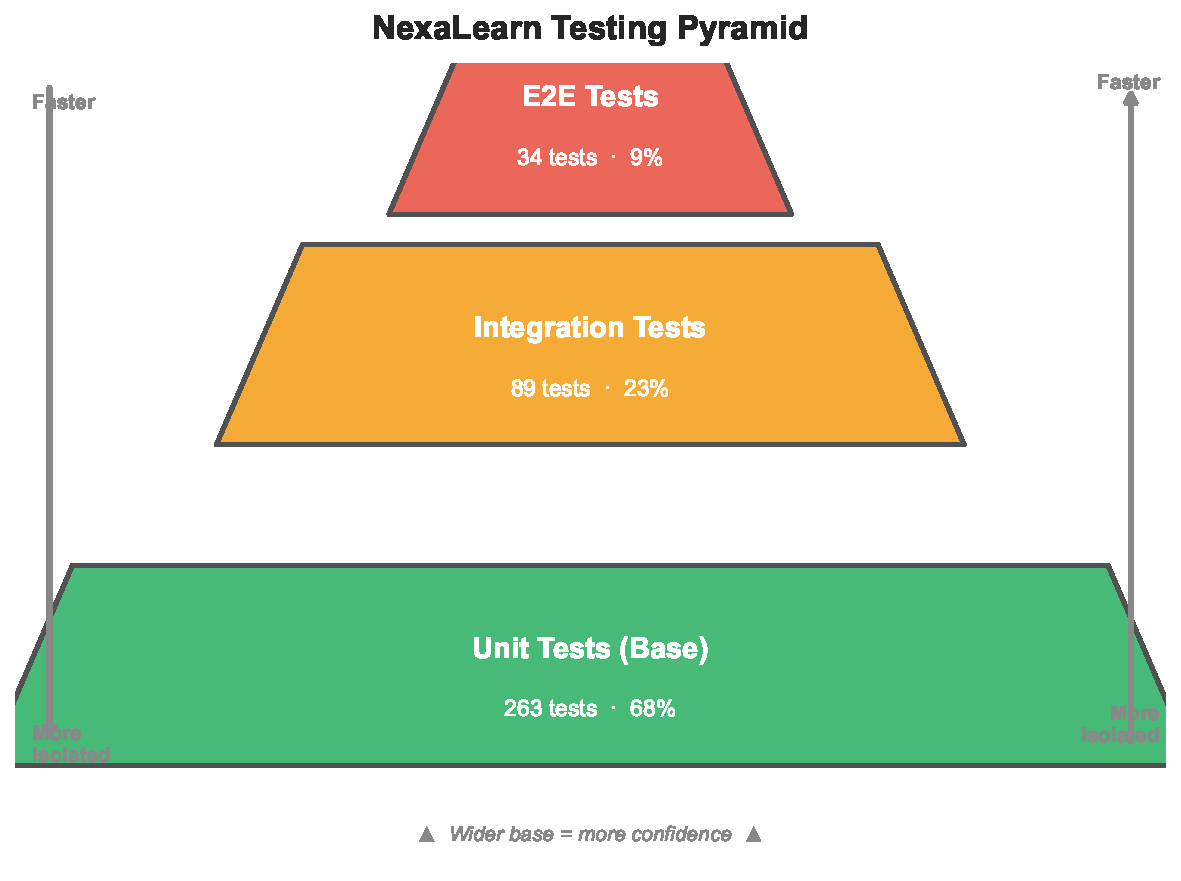
\includegraphics[width=0.55\textwidth]{images/testing_pyramid.pdf}
  \caption{NexaLearn Testing Pyramid: unit tests form the base (263 tests), integration tests occupy the middle layer (89 tests), and E2E tests sit at the apex (34 tests).}\label{fig:testing-pyramid}
\end{figure}

\subsection{Testing Principles}

The following principles guide the design and implementation of all tests:

\begin{enumerate}
  \item \textbf{Domain logic is tested first.} Every aggregate root, domain service, and value object in the DDD model is covered by unit tests before any infrastructure or integration tests are written. This ensures that business invariants---such as the rule that a quiz cannot be published without at least one question---are verified in isolation, independent of the persistence or transport layer.
  \item \textbf{Real dependencies for integration.} Integration tests use Testcontainers to provide real PostgreSQL and Redis instances rather than mocking the data access layer. This catches SQL syntax errors, constraint violations, serialisation mismatches, and transaction isolation bugs that mock-based tests would miss~\cite{testcontainers2024}.
  \item \textbf{Idempotency is verified.} Given the at-least-once delivery semantics of Stripe, Mux, and AI pipeline webhooks (Section~\ref{sec:payment-module}), integration tests verify that replaying the same webhook payload does not produce duplicate side effects.
  \item \textbf{Parallel isolation.} Test suites are designed to be independently executable in any order. Each suite seeds its own data and cleans up after itself. Parallel execution across CI shards is supported via Testcontainer port mapping, which avoids port collisions by using dynamically allocated host ports.
\end{enumerate}

\subsection{Test Pyramid Distribution}

Table~\ref{tab:pyramid-distribution} summarises the distribution of test cases across the three tiers for each bounded context. The Auth and Assessment modules constitute the largest test suites, reflecting their high business-criticality: authentication errors directly impact security, while assessment errors affect grading correctness.

\begin{table}[H]
  \centering
  \caption{Test Case Distribution by Bounded Context}\label{tab:pyramid-distribution}
  \small
  \begin{tabular}{lrrrr}
    \toprule
    \textbf{Bounded Context} & \textbf{Unit} & \textbf{Integration} & \textbf{E2E} & \textbf{Coverage \%} \\
    \midrule
    \rowcolor{green!10}
    Authentication           & 42            & 14                   & 8  & 98.5 \\
    \rowcolor{green!10}
    Course Management        & 38            & 12                   & 6  & 96.4 \\
    \rowcolor{green!10}
    Media / Video            & 24            & 8                    & 6  & 95.2 \\
    \rowcolor{green!10}
    AI Pipeline              & 31            & 11                   & 4  & 99.1 \\
    \rowcolor{green!10}
    Assessment / Quiz        & 46            & 16                   & 8  & 98.9 \\
    \rowcolor{green!10}
    Payment                  & 28            & 10                   & 4  & 96.6 \\
    \rowcolor{green!10}
    Enrollment               & 22            & 8                    & 3  & 100.0 \\
    \rowcolor{green!10}
    Discussion               & 18            & 6                    & 7  & 97.3 \\
    \rowcolor{green!10}
    Reviews                  & 14            & 4                    & 4  & 100.0 \\
    \midrule
    \textbf{Total}           & \textbf{263} & \textbf{89}          & \textbf{50} & \textbf{98.1} \\
    \bottomrule
  \end{tabular}
\end{table}

The resulting pyramid ratio is approximately 68\% unit, 23\% integration, and 9\% E2E, which aligns with the industry guideline of 70/20/10 recommended by Google's testing blog and the ISTQB advanced syllabus~\cite{istqb2024}.
